\chapter{Técnicas básicas}

Capítulo 3 de Szwarcfiter, \textit{Grafos e Algoritmos Computacionais}~\cite{Szwarcfiter1986grafos}.

%%%%%%%%%%%%%%%%%%%%%%%%%%%%%%%%%%%%%%%%%%%%%%%%%%%%%%%%%%%%
\section{Introdução}

Serão vistos neste capítulo alguns algoritmos básicos em grafos.

%%%%%%%%%%%%%%%%%%%%%%%%%%%%%%%%%%%%%%%%%%%%%%%%%%%%%%%%%%%%
\section{Ordenação topológica}

% Página 8

\begin{easylist}

  & Como visto na seção~\ref{sec:digraph}, sabemos que um digrafo acíclico $D(V, E)$ induz um conjunto parcialmente ordenado $(V, <)$. A relação $<$ é definida por $v < w \Leftrightarrow v$ alcança $w$ em $D$ para todo $v, w \in V$. Com isso, é possível ordenar os vértices do digrafo de modo a obter uma sequência $v1, \dots, v_n$, onde $n = |V|$ satisfazendo

  \[ v_i, < v_j \Rightarrow i<j \text{ para } i, j \in [1, n] \]

\begin{algorithm}[H]
\SetAlgoLined
\KwData{digrafo acíclico $D(V, E)$ }
 \For{ $j = 1, \dots, |V|$ }{
  escolher vértice $w$ com grau de entrada nulo\;
  remover $w$ de $V$\;
  $v_j \gets w$\;
 }
 \caption{Ordenação topológica em digrafo}
\end{algorithm}
  
\end{easylist}

%%%%%%%%%%%%%%%%%%%%%%%%%%%%%%%%%%%%%%%%%%%%%%%%%%%%%%%%%%%%
\section{Busca em árvores}

\clearpage

\begin{easylist}

  & Busca em árvores:
  
  && Busca em profundidade: visitamos primeiro a raiz. Do vértice atual, caso tenha filhos, visitamos seu primeiro filho não visitado; caso não tenha, retornamos para seu pai.

  && Busca em largura: visitamos primeiro a raiz. Colocamos os filhos do vértice atual em uma fila. Visitamos cada vértice da fila até que se esvazie.


  {\EXERCICIOS}
  
  \begin{enumerate}
  \item Considere a árvore abaixo. Em que ordem os vértices serão visitados pela primeira vez
    \begin{enumerate}
      \item em uma busca em profundidade?
      \item em uma busca em largura?
    \end{enumerate}
  \end{enumerate}

\begin{verbatim}

                                       a
                                      / \ 
                                     /   \
                                    /     \
                                   /       \
                                  /         \
                                 b           c
                                / \         /|\
                               /   \       / | \   
                              d     e     f  g  h
                             / \    |    /     / \
                            i   j   k   l     m   n

\end{verbatim}


  & Busca em grafos: em um grafo não há raiz, pai, filhos, direita, esquerda ou níveis, como em uma árvore. Para se ter controle dos vértices já visitados, evitando visitas múltiplas a um mesmo vértice, é necessário associar a cada vértice atributos ou marcas.

  && Busca em largura:

\begin{algorithm}[H]
\SetAlgoLined
\KwData{grafo conexo $G(V, E)$ }
  escolher, enfileirar e marcar vértice inicial arbitrário;

  \While{\textnormal{fila não vazia}}
  {
    $v \gets$ desenfileira();
    
    marcar e enfileirar vizinhos de $v$ não marcados;
  }
  \caption{Busca em largura em grafo}
\end{algorithm}

\clearpage

&& Busca em profundidade: visitamos primeiro a raiz. Do vértice atual, caso tenha filhos, visitamos seu primeiro filho não visitado; caso não tenha, retornamos para seu pai.

\end{easylist}


\begin{algorithm}[H]
\SetAlgoLined
\KwData{grafo conexo $G(V, E)$ }
  escolher vértice inicial arbitrário $v$;

  executar $P(v)$;

  \SetKwProg{Def}{def}{:}{end}
  \Def{$P(x)$}
  {
    marcar $x$\;
    empilhar $x$\;
    \For{$w \in \operatorname{adjacencia}(x)$}{
      \If{$w$ \textnormal{não é marcado}}
      { 
        $P(w)$;
      }
    }
    desempilhar $x$\;
  }
  \caption{Busca em profundidade em grafo}
\end{algorithm}

%%%%%%%%%%%%%%%%%%%%%%%%%%%%%%%%%%%%%%%%%%%%%%%%%%%%%%%%%%%%
\section{Busca irrestrita}

\begin{easylist}

  & Busca irrestrita: o algoritmo de busca irrestrita que veremos aqui é uma variação da busca em profundidade que permite que um mesmo vértice seja visitado várias vezes. Uma busca irrestrita em profundidade constrói uma árvore denominada árvore irrestrita de profundidade. A Figura~\ref{fig:3:1} mostra um exemplo desse tipo de árvore.

\end{easylist}


\begin{algorithm}[H]
\SetAlgoLined
\KwData{grafo conexo $G(V, E)$ }
  escolher vértice inicial arbitrário $v$;

  executar $P(v)$;

  \SetKwProg{Def}{def}{:}{end}
  \Def{$P(x)$}
  {
    marcar $x$\;
    empilhar $x$\;
    \For{$w \in \operatorname{adjacencia}(x)$}{
      \If{$w$ \textnormal{não é marcado}}
      { 
        $P(w)$;
      }
    }
    desempilhar $x$\;
    desmarcar $x$\;
  }
  \caption{Busca irrestrita em grafo}
\end{algorithm}


\begin{figure}[b]
  \begin{center}
    \begin{tabular}{c}
      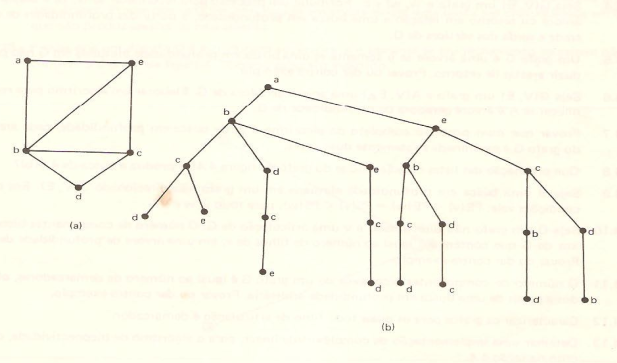
\includegraphics[width=0.7\textwidth]{images/03/unrestricted.png}
    \end{tabular}
  \end{center}
  \caption{\label{fig:3:1} (a) Um grafo $G(V,E)$; (b) árvore irrestrita de profundidade.}
  \source{Szwarcfiter~\cite{Szwarcfiter1986grafos}.}
\end{figure}
  





%%%%%%%%%%%%%%%%%%%%%%%%%%%%%%%%%%%%%%%%%%%%%%%%%%%%%%%%%%%%
%\section{Busca em árvores}


%%%%%%%%%%%%%%%%%%%%%%%%%%%%%%%%%%%%%%%%%%%%%%%%%%%%%%%%%%%%
%\section{Busca em grafos}


%%%%%%%%%%%%%%%%%%%%%%%%%%%%%%%%%%%%%%%%%%%%%%%%%%%%%%%%%%%%
%\section{Exercícios}

%\begin{enumerate}
%  \item 
%    \begin{enumerate}
%      \item 
%      \item 
%    \end{enumerate}
%  \item 
%  \item 
%\end{enumerate}

